\begin{surferIntroPage}{World Record Surfaces}{record_chmutovoktic}{משטחים שקבעו שיאי עולם}
    משטח מכונה \emph{לא-סינגולרי} או \emph{חלק} אם הוא אינו כולל שום קדקוד (קדקודים כאלה מכונים \emph{נקודות סינגולריות}). דוגמאות למשטחים חלקים הם ספֶרָה או טוֹרוּס, ראו שתי התמונות הראשונות
    משמאל להלן.  
    כאשר נבחר משטח רנדומלי, ברוב המקרים נבחר משטח חלק. 
 \begin{center}
      \vspace{-0,2cm}
      \begin{tabular}{@{}c@{}c@{}c@{\quad}c@{}c@{}c@{}c@{}}
        \begin{tabular}{@{}c@{}}
          חלק:
        \end{tabular}
        &
        \begin{tabular}{@{}c@{}}
          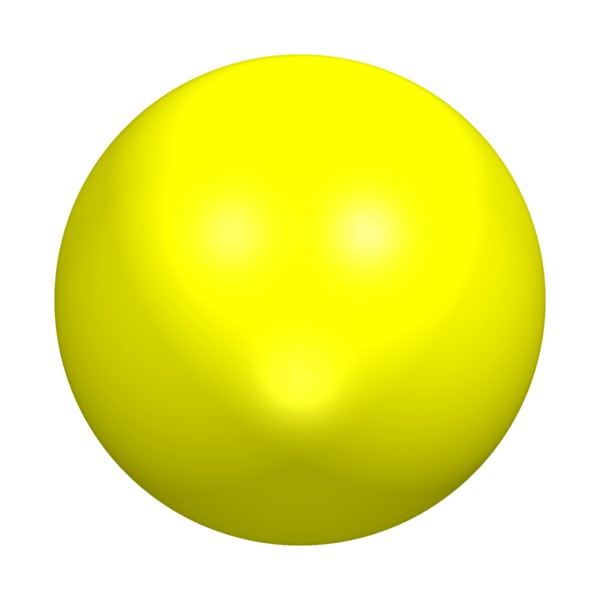
\includegraphics[width=1.1cm]{./../../common/images/kugel}
        \end{tabular}
        &
        \begin{tabular}{@{}c@{}}
          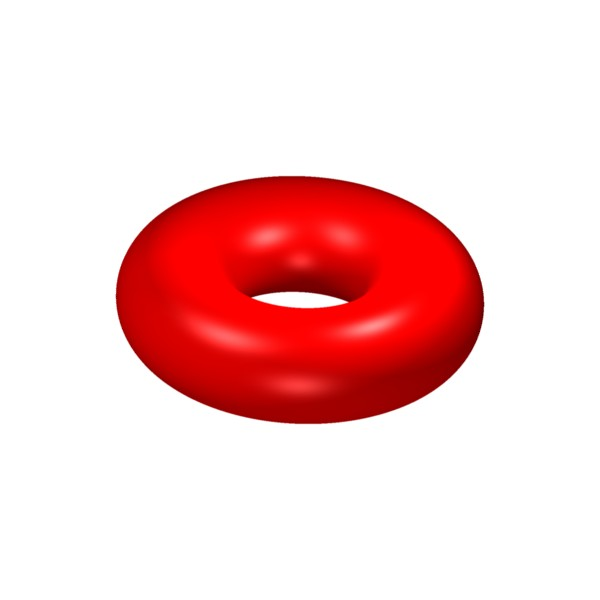
\includegraphics[width=1.1cm]{./../../common/images/torus}
        \end{tabular}
        &
        \begin{tabular}{@{}c@{}}
          נקודות סינגולריות\\
          רבות:
        \end{tabular}
        &
        \begin{tabular}{c@{}@{}}
          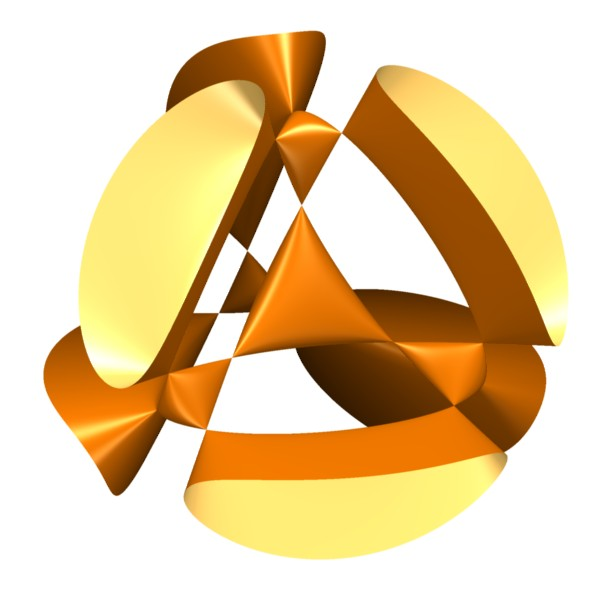
\includegraphics[width=1.1cm]{./../../common/images/kummer}
        \end{tabular}
        &
        \begin{tabular}{c@{}@{}}
          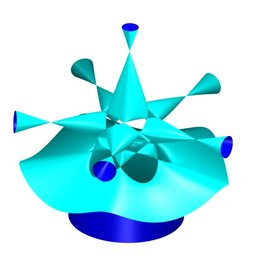
\includegraphics[width=1.1cm]{./../../common/images/togliatti}
        \end{tabular}
        &
        \begin{tabular}{c@{}@{}}
          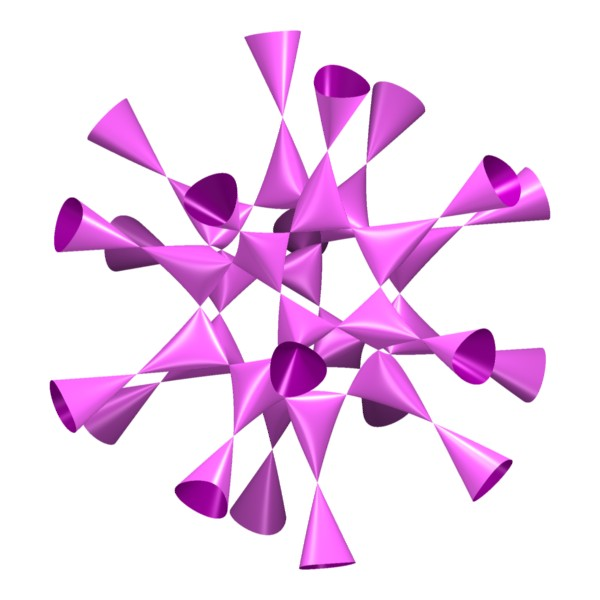
\includegraphics[width=1.1cm]{./../../common/images/barth_sextic}
        \end{tabular}
      \end{tabular}
    \end{center}
    \vspace{-0,2cm}
    לפיכך, כאשר משטח כולל נקודות סינגולריות, מדובר במקרה מיוחד מאד. אלה הן הנקודות המעניינות ביותר במשטח. המשטחים בתוכנת SURFER מוגדרים על-ידי פולינומים. החזקה הגבוהה ביותר של פולינום נקראת המעלה שלו $d$. מתמטיקאים שואלים כמה נקודות סינגולריות ייתכנו במשטח ממעלה מסוימת.
    נציין מספר זה בצורה הבאה: $\mu(d)$.

 מסתבר שקשה מאד לחשב את המספר $\mu(d)$.
    מאז המאה ה-$19$, $\mu(d)$ ידוע עבור משטחים ממעלה $d=1,2,3,4$, אך עבור $d=5$
    התגלה המספר רק בשנת 1980, ואילו עבור $d=6$ התגלה המספר המרבי של נקודות הסינגולריות רק בשנת 1996.
    ה-$\mu(d)$ עבור $d\ge 7$, עדיין לא ידוע.
  
    על כן, כל שיא עולם עבור $\mu(d)$ מסוים מהווה תוצאה חלקית חשובה. נראה שקשה מאד למצוא את הפתרון לבעיה זו כאשר מדובר ב-$d$ כלשהו.\\  לפניכם טבלה המסכמת מספר תוצאות ידועות:
    
   \begin{center}
      \begin{tabular}{r|cccccccc|c}
        $d$ & $1$ & $2$ & $3$ & $4$ & $5$ & $6$ & $7$ & $8$ & $d$\\
        \hline
        \hline
        \rule{0pt}{1.2em}$\mu(d)\ge$ & $0$ & $1$ & $4$ & $16$ & $31$ & $65$ &
        $99$ & $168$ & 
        $\approx \frac{5}{12}d^3$\\[0.3em]
        \hline
        \rule{0pt}{1.2em}$\mu(d)\le$ & $0$ & $1$ & $4$ & $16$ & $31$ & $65$ &
        $104$ & $174$ & $\approx \frac{4}{9}d^3$
      \end{tabular}
    \end{center}
\end{surferIntroPage}
